\section{System Overview}

The HILS scheme has two main programs that are built in a modular and
independent manner. This creates low coupling between the library and the two
main programs. In addition, we can choose whether or not the library will be
created in the compilation process so that we can save a little resources,
especially memory.

This researcher also built a library called ``hils-connector.'' There are two
libraries to be created, the C++ library for the GRS program on AGX/RKB
computers and the Python 3 library for the scenario runner program agent. The
Python library will be called a ``producer'' because it produces sensor data. C++
libraries will be called ``consumer'' because they consume sensor data. This
scheme utilizes sensor data and control/command data in a format sent from the
consumer to the producer after the sensor data has been successfully processed.
Then for the library features themselves, the libraries will directly
communicate with each other without using intermediaries. This makes the
solution simpler and reduces the overhead for communicating with intermediaries.
The library will also provide APIs for sending data and receiving data. To
support various types of sensors, the library will also have parsing,
serialization, and de-serialization features for GNSS, camera, and lidar
sensors.

The API provided by the ``producer'' library will directly consume sensor data
from CARLA so that library users do not need to make any modifications to
CARLA's sensor data. Likewise in the "consumer" library. The reverse API will be
customized so that library users can directly consume sensor data and directly
``feed'' it into NVIDIA DriveWorks virtual sensors. Then, to reduce various
additional overheads that can arise due to operation on the network, selected
communication mechanism using ZeroMQ.

ZeroMQ is a message queue so it is suitable for asynchronous operations in
accordance with sending sensor data from CARLA. Then, ZeroMQ is also very close
to TCP, but without the complexity of raw TCP. This is because one of ZeroMQ's
main goals is to reduce latency to as little as possible and maximize
throughput. ZeroMQ also doesn't have a broker, this is in accordance with the
desire to eliminate intermediaries so that producers and consumers can directly
communicate with each other. From the library solutions offered, a HILS system
architecture can be formed. This architecture can be seen in the deployment
diagram in Fig.~\ref{section-3-hils-deployment-diagram}.

\begin{figure}[htbp]
	\centerline{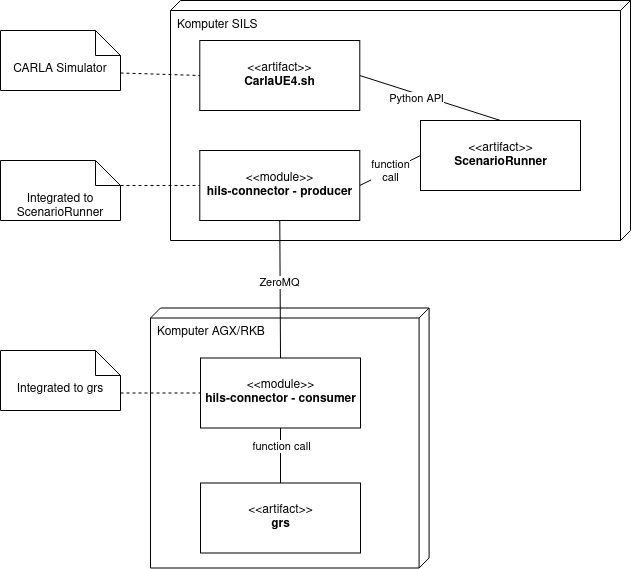
\includegraphics[width=0.4\textwidth]{chapter-3/deployment-diagram-new-hils.png}}
	\caption{HILS Scheme}
	\label{section-3-hils-deployment-diagram}
\end{figure}

\begin{table}[htbp]
	\caption{Table Type Styles}
	\label{tab1}
	\begin{center}
		\begin{tabular}{c c c c}
			\toprule
			\textbf{Table} & \multicolumn{3}{|c|}{\textbf{Table Column Head}}                                                         \\
			\cline{2-4}
			\textbf{Head}  & \textbf{\textit{Table column subhead}}           & \textbf{\textit{Subhead}} & \textbf{\textit{Subhead}} \\
			\midrule
			copy           & More table copy$^{\mathrm{a}}$                   &                           &                           \\
			\bottomrule
			\multicolumn{4}{l}{$^{\mathrm{a}}$Sample of a Table footnote.}
		\end{tabular}
	\end{center}
\end{table}